
	\chapter{Documentation of the Lamella Device for measuring lifetime statistics and thickness course simultaneously}
	
	\section{Description of the used color code}
	In \textcolor{red}{red} the communication from the display to the PSoC controller is written. 
	The receivable commands, which can be used for communication with a computer are written in \textcolor{blue}{blue}, the commands sendable to the computer are written in \textcolor{green}{green}.
	
	
%	\section{Planned for implementation}
%	\begin{itemize}
%		\item Change of file name (log of lifetime and intensity) via keyboard
%		\item Automatic enumeration of lamella lifetime log file via internal memory
%	\end{itemize}
%	
	
%	\section{Flow chart}
	
	\section{Software}

	\subsection{Home}
	\begin{figure}[h]
		\centering
		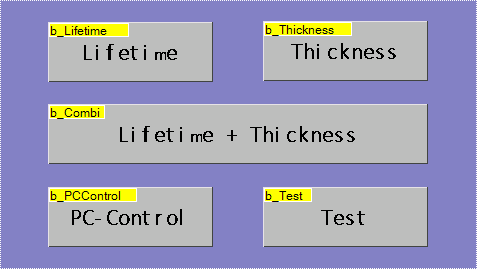
\includegraphics[width=0.7\linewidth]{LamellaDevice_Hardware/HomePage}
		\caption{Screenshot of the page ''Home''.}
		\label{fig:homepage}
	\end{figure}

	After turning on the device, all necessary hardware parts are initialised by the PSoC Controller. The end is indicated by switching to the ''Home'' screen shown in \ref{fig:homepage}.
	Here one can select, which measurement mode should be started. This is due to the fact, that not all measurement data is necessary for every measurement. 
	Additionally, the measurement parameter are chosen in such a way, that not too much time is wasted and not too much data garbage is created.
	
	An overview over the three measurements mode is given in Tab. \ref{tab:OverviewMeasurementModes}, but two more buttons are present. 
	The button ''PC-Control'' (\Nextion{P}) allows the controlling via serial communication and a script on the pc. This mode is present for special applications, in which the standard modi are not suited. It also allows the control of further I/O-pins of the PSoC Controller. 
	
	The button ''Test'' (\Nextion{Z}) opens a window in which the different hardware parts can be tested. 
	
	\subsection{Parameters}
	
	\subsubsection{Measurement Parameters}
	\begin{figure}[h]
		\centering
		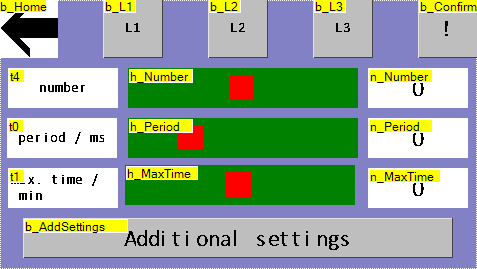
\includegraphics[width=0.7\linewidth]{LamellaDevice_Hardware/ParametersPage}
		\caption{Screenshot of the page ''Parameters''.}
		\label{fig:parameterspage}
	\end{figure}
	
	\begin{figure}[h]
		\centering
		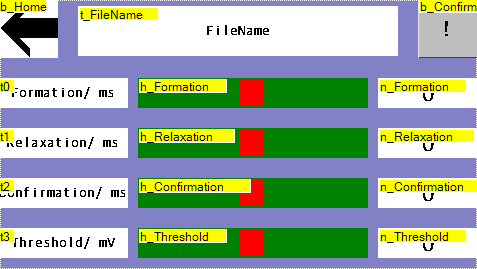
\includegraphics[width=0.7\linewidth]{LamellaDevice_Hardware/AddParametersPage}
		\caption{Screenshot of the page ''AddParameters''.}
		\label{fig:addsettingpage}
	\end{figure}


	All of the buttons for the three measurement modi opens the parameter page, shown in Fig. \ref{fig:parameterspage}, with the corresponding standard values. Here one can adjust the parameters as necessary.
	
	With the buttons ''L1'' (\Nextion{1}), ''L2'' (\Nextion{2}) and ''L3'' (\Nextion{3}) one can adjust, which laser(s) should be used for the measurement. Active lasers are indicated by a green button color, inactive ones by red color.
	The sliders for number (\Nextion{N}), period (\Nextion{P}) and max time (\Nextion{M}) are used for setting the parameters.
	
	With the button ''Additional settings'' (\Nextion{X}) a second parameter window opens, seen in Fig. \ref{fig:addsettingpage}.
	Here the sliders are used for setting the formation time (\Nextion{F}), relaxation time (\Nextion{R}), confirmation time (\Nextion{C}) and threshold value (\Nextion{T}). 
	The button ''!'' (\Nextion{X}) is used for confirmations of the settings and switching back to the first parameter window. 
	
	The initialisation for receiving slider values is done with the character \Nextion{\&}.
	
	\begin{table}[h]
		\centering
		\label{tab:OverviewMeasurementModes}
		\caption{Overview over the different measurement modes. \\ *: Minimum time for correct writing to SD-Card.}
		\begin{tabular}{|c|c|c|c|}
			\hline 
			Button & Lifetime & Thickness & Lifetime+Thickness \\ 
			\hline 
			Serial Command: & \textcolor{red}{L} & \textcolor{red}{T} & \textcolor{red}{C} \\ 
			\hline 
			Number of Measurements & 300 & 50 & 300 \\ 
			\hline 
			Period for Laser Switch / \SI{}{\milli\second} & 50 & 500* & 500* \\ 
			\hline 
			Maximum Measurement Time / \SI{}{\min} & 300 & 60 & 300 \\ 
			\hline 
			Formation Time / \SI{}{\milli\second} & 5000 & 5000 & 5000 \\ 
			\hline 
			Relaxation Time / \SI{}{\milli\second} & 5000 & 5000 & 5000 \\ 
			\hline 
			Confirmation Time / \SI{}{\milli\second} & 5000 & 5000 & 5000 \\ 
			\hline 
			Threshold Value / \SI{}{\milli\volt} & 55 & 55 & 55 \\ 
			\hline 
			Datalogging & False & True & True \\ 
			\hline 
		\end{tabular} 
	\end{table}
	
	\subsubsection{Filename (not working right now)}
	
	\begin{figure}[h]
		\centering
		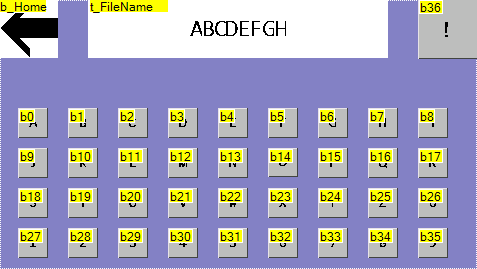
\includegraphics[width=0.7\linewidth]{LamellaDevice_Hardware/FileNamePage}
		\caption{Screenshot of the page ''FileName''.}
		\label{fig:filename}
	\end{figure}


	The buttons seen in Fig. \ref{fig:filename} are sending the corresponding \Nextion{lower case letter} to the PSoC. 

	
	\subsection{Setup}
	
	\begin{figure}[h]
		\centering
		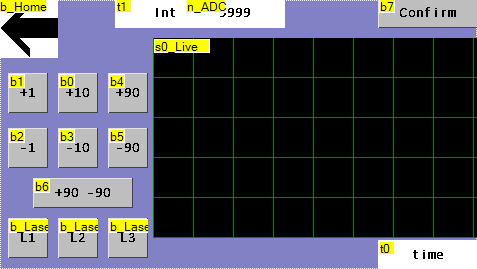
\includegraphics[width=0.7\linewidth]{LamellaDevice_Hardware/SetupPage}
		\caption{Screenshot of the page ''Setup''.}
		\label{fig:setuppage}
	\end{figure}
	
	After setting the parameters by confirmation with the ''!'' button in the first parameter window, the PSoC switches to the setup page, shown in Fig. \ref{fig:setuppage}. 
	This page is used for orientation of the metal frame, so that the measured intensity is at the maximum.
	For this, the step motor can be rotated by the present buttons. An overview over them is given in Tab \ref{tab:OverviewSetupButtons}, additionally the three usable lasers can be turned on and off, with the buttons ''L1'' (\Nextion{1}), ''L2'' (\Nextion{3}) and ''L3'' (\Nextion{3}). In the top the most recent measured intensity is written. 
	The graphic on the right side shows the last intensity measurements for determining the efficiency of rotating the step motor. \\
	For better readability the intensity is only measured every \SI{100}{\milli\second}. 
	After reaching the maximum of the measureable intensity, the measurements are started with the button ''Confirm'' (\Nextion{O}). 
	\begin{table}[h]
		\centering
		\label{tab:OverviewSetupButtons}
		\caption{Overview over the buttons for controlling the step motor on the page ''Setup''. Here is ''CW'' the abbreviation for ''clockwise'' and ''CCW'' for ''counterclockwise''}
		\begin{tabular}{|c|c|c|c|}
			\hline 
			Button & Direction & Action & Serial Command \\ 
			\hline 
			+1 & CW & 1 Step & \textcolor{red}{+} \\ 
			\hline 
			-1 & CCW & 1 Step & \textcolor{red}{-} \\ 
			\hline 
			+10 & CW & 10 Degree & \textcolor{red}{.} \\ 
			\hline 
			-10 & CCW & 10 Degree & \textcolor{red}{,} \\ 
			\hline 
			+90 & CW & 90 Degree & \textcolor{red}{!} \\ 
			\hline 
			-90 & CCW & 90 Degree & \textcolor{red}{?} \\ 
			\hline 
			+90 -90 & CW + CCW & 90 Degree + 90 Degree  & \textcolor{red}{\#} \\ 
			\hline 
		\end{tabular} 
	\end{table}
	
	\subsection{Measurement}
	
	This page, shown in Fig.  \ref{fig:measurementpage}, gives an overview over the measured data. In the top a progress bar with the recent and planned lamella number is given. The button ''Stop'' (\Nextion{S}) can be used for stopping the measurement earlier than planned. 
	For controlling if the device has stopped, the data for the timer and the intensity in the top right corner is refreshed every \SI{500}{\milli\second}. 
	In order to see the previously measured lifetimes (and for estimating the finishing time manually) the graph shows a section of the measured lifetimes. 

	
	\begin{figure}[h]
		\centering
		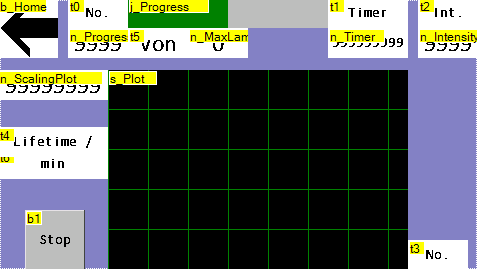
\includegraphics[width=0.7\linewidth]{LamellaDevice_Hardware/MeasurementPage}
		\caption{}
		\label{fig:measurementpage}
	\end{figure}
	
	
	
	
%	\subsection{PC-Control (not working right now)}
%
%	\begin{figure}[h]
%		\centering
%		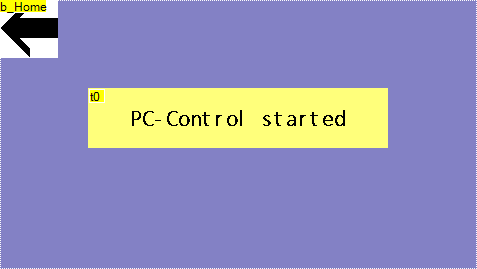
\includegraphics[width=0.7\linewidth]{PCControlPage}
%		\caption{Screenshot of the page ''PCControl''.}
%		\label{fig:pccontrolpage}
%	\end{figure}
%
%	Fig. \ref{fig:pccontrolpage} shows a screenshot of the page ''PCControl''. For controlling via a computer it is necessary to establish a serial connection over the USB-port of the device, with a BAUD rate of 115200bps. 
%	
%	A received signal triggers the interrupt function and the following interpretation of the signal according to table \ref{tab:ReceivingCommands}. 
%	
%	The signal used for answering the requests from the computer are given in table \ref{tab:SendingCommands}. 
%	
%\begin{table}[h]
%	\centering
%	\label{tab:ReceivingCommands}
%	\caption{Overview over the serial commands, which can be interpreted from the PSoC. Here stands CW for clockwise and CCW for counterclockwise. }
%	
%	\begin{tabular}{|c|c|}
%		\hline 
%		Serial Command & Function \\ 
%		\hline 
%		\FromPC{+} & Move stepper one step CW \\ 
%		\hline 
%		\FromPC{-} & Move stepper one step CCW \\ 
%		\hline 
%		\FromPC{.} & Move stepper 10 degree CW\\ 
%		\hline 
%		\FromPC{,} & Move stepper 10 degree CCW \\ 
%		\hline 
%		\FromPC{!} & Move stepper 90 degree CW \\ 
%		\hline 
%		\FromPC{?} & Move stepper 90 degree CCW \\ 
%		\hline
%		\hline 
%		\FromPC{1} & Toggle laser 1, returns new state (\ToPC{1} or \ToPC{0})\\ 
%		\hline 
%		\FromPC{2} & Toggle laser 2, returns new state (\ToPC{1} or \ToPC{0})\\ 
%		\hline 
%		\FromPC{3} & Toggle laser 3, returns new state (\ToPC{1} or \ToPC{0})\\ 
%		\hline 
%		\hline
%		\FromPC{8} & Toggle output 1, returns new state (\ToPC{1} or \ToPC{0})\\
%		\hline
%		\FromPC{9} & Toggle output 2, returns new state (\ToPC{1} or \ToPC{0})\\
%		\hline
%		\hline
%		\FromPC{R} & Resets lifetime timer  \\ 
%		\hline
%		\hline 
%		\FromPC{M} & \shortstack{Requests measurement data in form: \\ \ToPC{Laserstates-timer-ADCValue} \\e.g. \ToPC{100-1000-253}}  \\ 
%		\hline 
%		\FromPC{T} & Requests recent ADC-value.\\
%		\hline
%		\hline
%		\FromPC{H} & \shortstack{Stops execution of Serial Commands\\ and switches to ''Home'' screen}\\
%		
%		\hline
%	\end{tabular} 
%	\end{table}
%
%
%
%	\begin{table}[h]
%		\centering
%	\label{tab:SendingCommands}
%\caption{Overview over the serial commands, which the PSoC sends. }
%		
%		\begin{tabular}{|c|c|}
%			\hline 
%			Serial Command & Function \\ 
%			\hline 
%			\ToPC{\#} & Confirm execution of received command\\ 
%			\hline
%			\ToPC{.} & Command not programmed, will be ignored. \\			
%			\hline
%			\shortstack{\ToPC{Laserstates-timer-ADCValue} \\
%				e.g. \ToPC{100-1000-253} }& \shortstack{Answer to request of \\
%				measurement data by \FromPC{M}} \\
%			\hline 
%		\end{tabular} 
%	\end{table}
%
%	\newpage

	\subsection{Test}
	
	\begin{figure}[h]
		\centering
		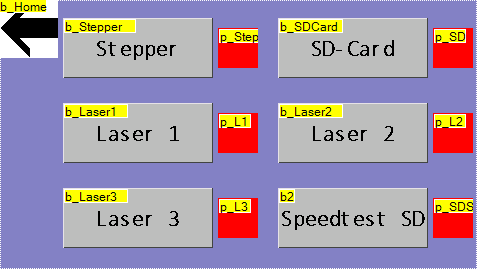
\includegraphics[width=0.7\linewidth]{LamellaDevice_Hardware/TestPage}
		\caption{Screenshot of the page ''Test''.}
		\label{fig:testpage}
	\end{figure}

	With the three buttons ''Laser1'' (\Nextion{1}), ''Laser2'' (\Nextion{2}) and ''Laser3'' (\Nextion{3}) the lasers can be turned off and on. Corresponding to the actual state the color of the field besides it changes from red (OFF) to green (ON) and vice versa.
	The button ''Step Motor'' (\Nextion{M}) starts the rotation of the motor by 90 Degree clockwise, and afterwards 90 Degree counterclockwise, the end is indicated by a green colored field.
	The functionality of the SD-Card can be tested by the buttons ''SD-Card'' (\Nextion{C}) and ''Speedtest SD'' (\Nextion{S}). 
	
	\section{Hardware}
	
	\subsection{Pinout}
	\begin{tabular}{|c|c|}
			\hline
			Pin & Function \\	
			\hline
			0.4 & Input for detector\\
			\hline
			\hline
			1.2 & Output 2 \\
			\hline
			1.4 & Output 1 \\
			\hline
			\hline
			1.5 & Laser 3 \\
			\hline
			\hline
			1.6 & TX for computer \\
			\hline
			1.7 & RX for computer \\
			\hline
			\hline
			2.4 & LED (indicates Init-process) \\
			\hline
			2.5 & LED (unused) \\
			\hline
			2.6 & LED (unused) \\
			\hline
			2.7 & LED (unused) \\
			\hline
			\hline
			3.0 & Pin for Stepper (direction) \\
			\hline
			3.1 & Pin for Stepper (CLK) \\
			\hline
			3.2 & Pin for Stepper (SLEEP) \\
			\hline
			3.3 & Pin for Stepper (RES) \\
			\hline
			3.4 & Pin for Stepper (MS3) \\
			\hline
			3.5 & Pin for Stepper (MS2) \\
			\hline
			3.6 & Pin for Stepper (MS1) \\
			\hline
			3.7 & Pin for Stepper (EN) \\
			\hline
			\hline
			12.0 & Laser 1 \\
			\hline
			12.1 & Laser 2 \\
			\hline
			\hline
			12.2 & Indication of Measurement \\
			\hline
			\hline
			12.4 & RX for Nextion Display \\
			\hline
			12.5 & TX for Nextion Display \\
			\hline
			
		\end{tabular}
	
	
	\section{Error Codes}
		\begin{tabular}{|c|c|}
			\hline 
			Code & Problem \\ 
			\hline 
			1 & Wrong Interrupt from Nextion Display received.\\
			\hline
			\hline
			100 & No laser is activated for measurement \\ 
			\hline 
			101 & No measurement mode is selected \\
			\hline
			\hline
			700 & File for lifetime logging could not be opened. \\ 
			\hline 
			701 & Write of lifetime to file failed.   \\ 
			\hline 
			702 & File for lifetime logging could not be closed. \\ 
			\hline 
			710 & File for speedtest logging could not be opened. \\ 
			\hline 
			711 & Write of speedtest data to file failed.   \\ 
			\hline 
			712 & File for speedtest logging could not be closed. \\ 
			\hline 		
			720 & File for intensity logging could not be opened. \\ 
			\hline 
			721 & Write of intensity value to file failed.   \\ 
			\hline 
			722 & File for intensity logging could not be closed. \\ 
			\hline 
		\end{tabular} 
	
%	\section{Source Code}
%	\subsection{Nextion-Display}
%		\subsubsection{Variable: g\_activePage}
%			\begin{tabular}{|c|c|}
%			\hline
%			Character & Page \\
%			\hline
%			H & Home \\
%			\hline
%			E & Error \\
%			\hline
%			Z & Test \\
%			\hline
%			S & Measurement-Setup \\
%			\hline
%			M & Measurement \\
%			\hline
%			F & Finished \\
%			\hline
%			C & Measurement-Configuration \\
%			\hline
%			L & LaserSelect \\
%			\hline
%			A & Filename \\
%			\hline
%			\end{tabular}
		